\documentclass[11pt,a4paper,onside,UTF8]{article}
\usepackage{geometry}
	\geometry{left=2cm,right=2cm,top=2.5cm,bottom=3cm}
\usepackage[utf8]{inputenc}
\usepackage[english]{babel}
\usepackage{lipsum}
\usepackage{bm}
\usepackage{upgreek}

\usepackage{amsmath}
% mathtools for: Aboxed (put box on last equation in align envirenment)
\usepackage{microtype} %improves the spacing between words and letters

\usepackage{xeCJK,paralist,enumerate,booktabs,multirow,graphicx,float,setspace}
	\setlength{\parindent}{2em}%正文首行缩进两个汉字
% \usepackage{ctex}
%     \setmainfont{Times New Roman}

%% COLOR DEFINITIONS

\usepackage[svgnames]{xcolor} % Enabling mixing colors and color's call by 'svgnames'

\definecolor{MyColor1}{rgb}{0.2,0.4,0.6} %mix personal color
\newcommand{\textb}{\color{Black} \usefont{OT1}{lmss}{m}{n}}
\newcommand{\blue}{\color{MyColor1} \usefont{OT1}{lmss}{m}{n}}
\newcommand{\blueb}{\color{MyColor1} \usefont{OT1}{lmss}{b}{n}}
\newcommand{\red}{\color{LightCoral} \usefont{OT1}{lmss}{m}{n}}
\newcommand{\green}{\color{Turquoise} \usefont{OT1}{lmss}{m}{n}}

\DeclareMathOperator{\trace}{trace}
\DeclareMathOperator{\diag}{diag}

%% FONTS AND COLORS

%    SECTIONS

\usepackage{titlesec}
	\newfontfamily\sectionef{Times New Roman}
	\setCJKfamilyfont{FZHeiTi}{黑体}
	\newcommand{\sectioncf}{\CJKfamily{FZHeiTi}}
	\titleformat*{\section}{\large\bfseries\sectioncf\sectionef}
	\titleformat*{\subsection}{\normalsize\bfseries\sectioncf\sectionef}
\usepackage{sectsty}
%%%%%%%%%%%%%%%%%%%%%%%%
%set section/subsections HEADINGS font and color
\sectionfont{\color{MyColor1} \usefont{OT1}{lmss}{b}{n}}  % sets colour of sections
\subsectionfont{\color{MyColor1}\usefont{OT1}{lmss}{b}{n}}  % sets colour of sections

%set section enumerator to arabic number (see footnotes markings alternatives)
\renewcommand\thesection{\arabic{section}.} %define sections numbering
\renewcommand\thesubsection{\thesection\arabic{subsection}} %subsec.num.

%define new section style
\newcommand{\mysection}{
\titleformat{\section} [runin] {\usefont{OT1}{lmss}{b}{n}\color{MyColor1}} 
{\thesection} {3pt} {} } 


%	CAPTIONS
\usepackage{caption}
\usepackage{subcaption}
%%%%%%%%%%%%%%%%%%%%%%%%
% \captionsetup[figure]{labelfont={color=Turquoise}}


%		!!!EQUATION (ARRAY) --> USING ALIGN INSTEAD
%using amsmath package to redefine eq. numeration (1.1, 1.2, ...) 
\renewcommand{\theequation}{\thesection\arabic{equation}}



\makeatletter
\let\reftagform@=\tagform@
\def\tagform@#1{\maketag@@@{(\ignorespaces\textcolor{red}{#1}\unskip\@@italiccorr)}}
\renewcommand{\eqref}[1]{\textup{\reftagform@{\ref{#1}}}}
\makeatother
\usepackage[colorlinks,linkcolor=blue,urlcolor=blue]{hyperref}%超链接

% For labeling top of page on every page but first one:
\usepackage{fancyhdr}

% PREPARE TITLE:
\title{\blue Medical Statistics \\
\blueb Homework 2}
\author{实验2班 ~~ 莫润冰 ~~ 20980131}
\date{}

\renewcommand{\rmdefault}{phv} % Arial Font
\renewcommand{\sfdefault}{phv} % Arial Font
\usepackage{datetime}

\pagestyle{fancy}
\fancyhead{}
% \fancyhead[CO,CE]{{\small{{\bf{Homework Number}} - Class Name - Semester - Your Name}}}
\fancyhead[L]{Medical Statistics}
\fancyhead[R]{\shortmonthname[\the\month], \the\year}
\fancyhead[C]{
\normalsize{HW1}
}

\usepackage{listings}
\usepackage{color}

\definecolor{dkgreen}{rgb}{0,0.6,0}
\definecolor{gray}{rgb}{0.5,0.5,0.5}
\definecolor{mauve}{rgb}{0.58,0,0.82}

\lstset{ %
	language=R,                % the language of the code
	basicstyle={\footnotesize\usefont{OT1}{lmss}{m}{n}},           % the size of the fonts that are used for the code
	numbers=left,                   % where to put the line-numbers
	numberstyle=\tiny\color{gray},  % the style that is used for the line-numbers
	stepnumber=1,                   % the step between two line-numbers. If it's 1, each line 
									% will be numbered
	numbersep=5pt,                  % how far the line-numbers are from the code
	backgroundcolor=\color{white},      % choose the background color. You must add \usepackage{color}
	showspaces=false,               % show spaces adding particular underscores
	showstringspaces=false,         % underline spaces within strings
	showtabs=false,                 % show tabs within strings adding particular underscores
	frame=single,                   % adds a frame around the code
	rulecolor=\color{black},        % if not set, the frame-color may be changed on line-breaks within not-black text (e.g. commens (green here))
	tabsize=2,                      % sets default tabsize to 2 spaces
	captionpos=b,                   % sets the caption-position to bottom
	breaklines=true,                % sets automatic line breaking
	breakatwhitespace=false,        % sets if automatic breaks should only happen at whitespace
	title=\lstname,                   % show the filename of files included with \lstinputlisting;
									% also try caption instead of title
	keywordstyle=\color{red},          % keyword style
	commentstyle=\color[cmyk]{1,0,1,0},       % comment style
	stringstyle=\color{MyColor1},         % string literal style
	escapeinside={\%*}{*)},            % if you want to add LaTeX within your code
	morekeywords={*,...}               % if you want to add more keywords to the set
}



%%%%%%%%%%%%%%%%%%%%%%%%%%%%%%%%%%%%%%%%%%%%%%%%%%%%%%%%%%%%%%%%%%%%%%%%%%%%%%%%%%%%%%%
%%%%%%%%%%%%%%%%%%%%%%%%%%%%%%%%%%%%%%%%%%%%%%%%%%%%%%%%%%%%%%%%%%%%%%%%%%%%%%%%%%%%%%%
\begin{document}
\maketitle

\renewcommand{\thefootnote}{\fnsymbol{footnote}}
\footnotetext[1]{Github repo: \url{https://github.com/MoRunbing/Medical_Statistics }}
\footnotetext[2]{E-mail: \url{morb@mail2.sysu.edu.cn}}

\section{Exercise 1}

\begin{figure}[H]
	\centering
	\subfloat[]{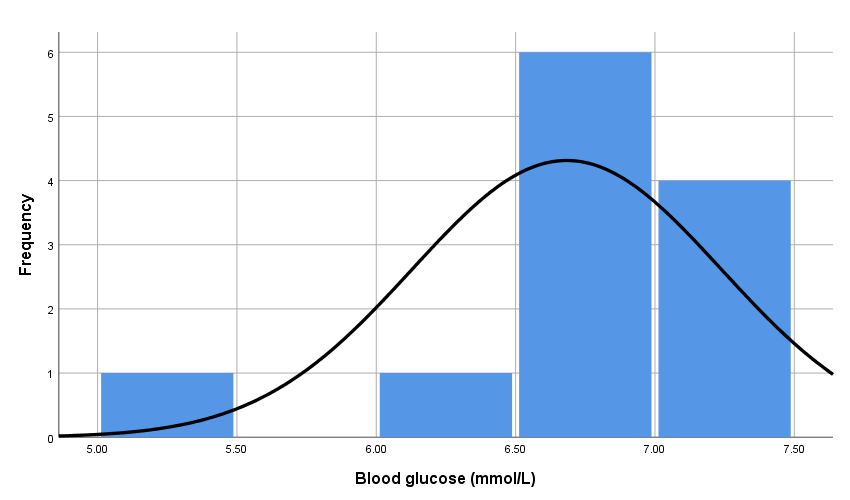
\includegraphics[width=0.5\textwidth]{fig//hist.png}}
	\subfloat[]{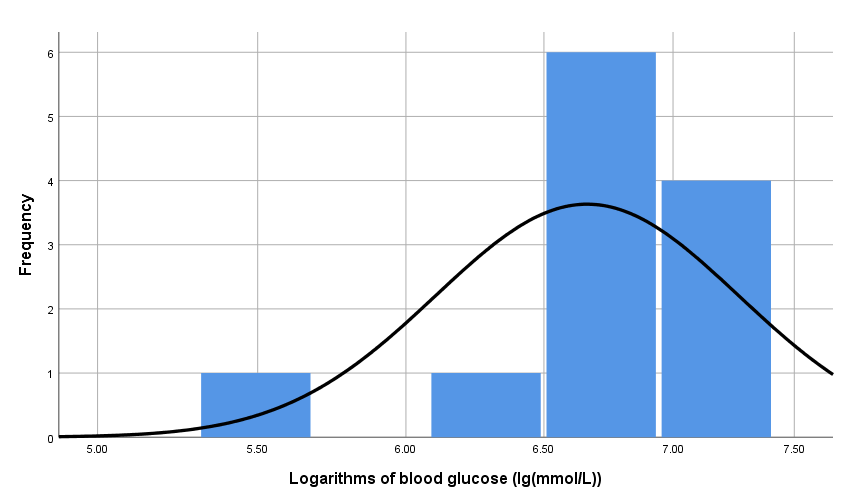
\includegraphics[width=0.5\textwidth]{fig//hist_lg.png}}
	\caption{Histogram of blood glucose level of 12 random patients}
\end{figure}
The blood glucose level is a continous value. The histogram is higher around the center and shorter on two sides but not symmetric.
The tail on the negative side is much longer than the positive side, so it is called a negative skew. 

\subsection{Measurement of Average}

\begin{equation}
	arithmetic \ mean: \bar{x} = \frac{1}{n}\sum_{i = 1}^{n} x_i = 6.683
\end{equation}
\begin{equation}
	geometric \ mean: \bar{x}= \sqrt[n]{x_1 x_2 \cdots x_n} = 6.661
\end{equation}
\begin{equation}
	median: M_d = 6.685
\end{equation}
*total number of patients n = 12; $x_i$ represents the blood glucose level of $i^{th}$ patient
\\ \hspace*{\fill} \\

The minimum value 5.31 is far from average value compared to others, so the arithmetic mean is not suitable for measuring average.
The logarithmic histogram of blood glucose is not close to a normal distribution, so the geometric mean is not suitable as well.
Since the histogram is taller around the center and shorter on two sides, and it is a negative skew, so median can best present the average level. 

\subsection{Measurement of Variation}

\begin{equation}
	maximum\ value = 7.35
\end{equation}
\begin{equation}
	minimum\ value = 5.31
\end{equation}
\begin{equation}
	range = maximum\ value - minimum\ value = 2.04
\end{equation}

\begin{equation}
	Q_3 = 7.125
\end{equation}
\begin{equation}
	Q_1 = 6.530
\end{equation}
\begin{equation}
	Q_3-Q_1 = 0.595
\end{equation}

\begin{equation}
	standard\ deviation: S = \sqrt{S^2} = 0.555
\end{equation}

$Q_3-Q_1$ discribes sample variance better than range since it excludes those extreme values. 
Also, the histogram is a negative skew rather than a normal distribution, so $Q_3-Q_1$ best reflects the variation.

\section{Exercise 2}
\begin{figure}[H]
	\centering
    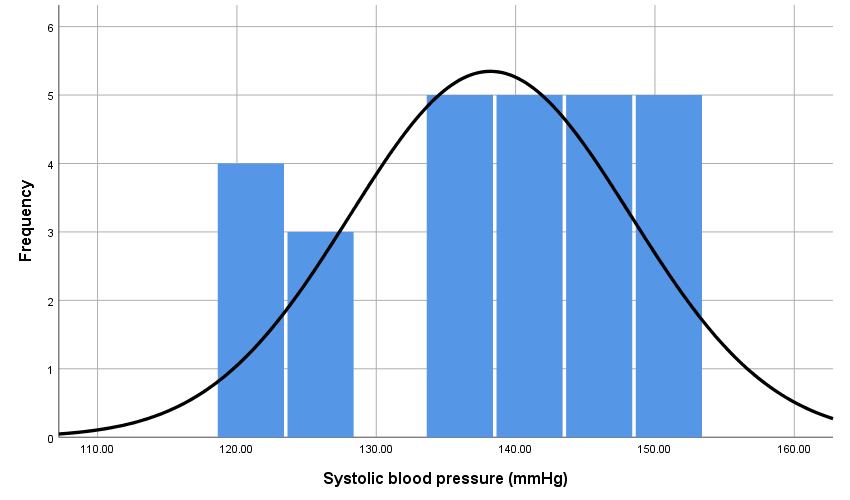
\includegraphics[width=0.7\textwidth]{fig//hist2.png}
	\caption{Histogram of systolic blood pressure (mmHg)}
\end{figure}

The systolic blood pressure is a continous value. The distribution curve is higher around the center and shorter on two sides.
Also, it is symmetric, so it is close to a normal distribution.
Usually, we choose arithmetic mean to reflect the average and standard deviation to reflect the variation of the data
which is close to a normal distribution.

\begin{equation}
	arithmetic \ mean: \bar{x} = \frac{1}{n}\sum_{i = 1}^{n} x_i = 138.185
\end{equation}
\begin{equation}
	standard\ deviation: S = \sqrt{S^2} = 10.073
\end{equation}
*total number of collected systolic blood pressure n = 27; $x_i$ represents the $i^{th}$ systolic blood pressure
\\ \hspace*{\fill} \\

So the systolic blood pressure can be described as $138.185 \pm 10.073$ mmHg. 
\end{document}